\documentclass[12pt,a4paper]{article}
\usepackage[utf8]{inputenc}
\usepackage[T1]{fontenc}
\usepackage{amsmath}
\usepackage{geometry}
\usepackage{setspace}
\usepackage{parskip}
\usepackage{enumitem}
\usepackage{booktabs}
\usepackage{longtable}
\usepackage{array}
\usepackage{xcolor}
\usepackage{hyperref}
\usepackage{float}
\usepackage{tikz}
\usetikzlibrary{arrows.meta,positioning,calc,matrix}
\usepackage{fancyhdr}
\usepackage{titlesec}

\geometry{left=2.5cm,right=2.5cm,top=2.5cm,bottom=2.5cm,headheight=14.5pt}
\onehalfspacing
\hypersetup{colorlinks=true,linkcolor=black,urlcolor=blue,pdftitle={Sistema Integral de Gestión de Eventos},pdfauthor={Daniel Cristancho, Samuel Emperador, Sebastián Sánchez, Diego Coronado}}

\definecolor{azul}{RGB}{31,78,121}
\definecolor{gris}{RGB}{242,242,242}
\definecolor{grisoscuro}{RGB}{80,80,80}
\definecolor{verde}{RGB}{39,120,70}
\definecolor{naranja}{RGB}{230,126,34}
\definecolor{morado}{RGB}{106,27,154}

\titleformat{\section}{\Large\bfseries\color{azul}}{\thesection.}{0.5em}{}
\titleformat{\subsection}{\large\bfseries}{\thesubsection.}{0.5em}{}
% Etiquetas en español (sin babel, que no está disponible en este entorno)
\renewcommand{\contentsname}{Índice}
\renewcommand{\figurename}{Figura}
\renewcommand{\tablename}{Tabla}

\pagestyle{fancy}
\fancyhf{}
\fancyhead[L]{Sistema Integral de Gestión de Eventos}
\fancyhead[R]{Arquitectura de Software}
\fancyfoot[C]{\thepage}

\begin{document}

\begin{titlepage}
\centering
\vspace*{2cm}
{\Huge\bfseries Sistema Integral de Gestión de Eventos\par}
\vspace{0.7cm}
{\Large Arquitectura de Software\par}
\vspace{1.2cm}
{\Large\bfseries Atributos de Calidad y Propuesta Arquitectónica\par}
\vspace{2cm}
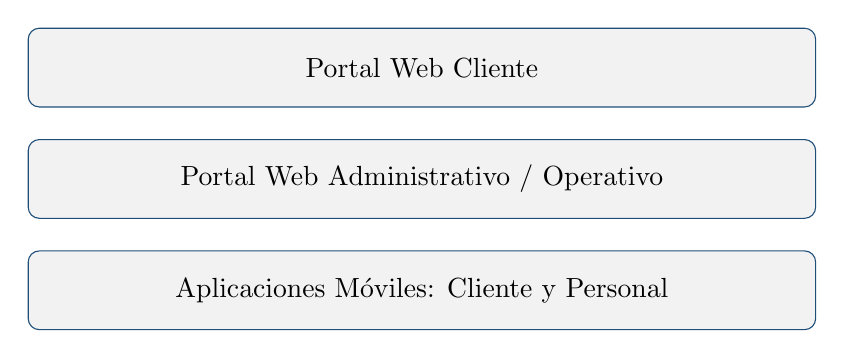
\begin{tikzpicture}
\node[draw=azul,rounded corners,fill=gris,minimum width=10cm,minimum height=1cm,align=center]
{Portal Web Cliente};
\node[draw=azul,rounded corners,fill=gris,minimum width=10cm,minimum height=1cm,below=0.4cm of current bounding box.south,align=center]
{Portal Web Administrativo / Operativo};
\node[draw=azul,rounded corners,fill=gris,minimum width=10cm,minimum height=1cm,below=0.4cm of current bounding box.south,align=center]
{Aplicaciones Móviles: Cliente y Personal};
\end{tikzpicture}
\vfill
\begin{tabular}{rl}
\textbf{Materia:} & Arquitectura de Software\\
\textbf{Integrantes:} & Daniel Cristancho, Samuel Emperador, Sebastián Sánchez, Diego Coronado\\
\textbf{Fecha:} & Agosto de 2026
\end{tabular}
\end{titlepage}

\tableofcontents
\newpage

\section{Introducción}

Este documento presenta una segunda versión del análisis de atributos de calidad y de la propuesta de arquitectura para el \textbf{Sistema Integral de Gestión de Eventos}. La propuesta toma como base la primera versión del proyecto, donde se planteó una organización mediana-grande que gestiona eventos masivos, como conciertos, festivales y partidos deportivos, con miles de usuarios concurrentes, especialmente durante la apertura de venta y el ingreso al recinto.

El sistema centraliza procesos de boletería, mercado secundario de entradas, administración de personal, parqueaderos y operación de eventos. En esta segunda versión se define con mayor precisión la distribución de funcionalidades entre las interfaces.

Se contemplan cuatro clientes principales:

\begin{itemize}
\item \textbf{Portal Web del Cliente:} compra, consulta y gestión de entradas, reventas, promociones y parqueaderos.
\item \textbf{Portal Web Administrativo y Operativo:} utilizado por administradores, organizadores y trabajadores autorizados.
\item \textbf{Aplicación Móvil del Cliente:} principalmente para visualizar entradas y códigos QR, información y notificaciones.
\item \textbf{Aplicación Móvil del Personal:} para turnos, asistencia, instrucciones, reportes y alertas.
\end{itemize}

La primera propuesta priorizó consistencia, disponibilidad, seguridad y rendimiento. Esta versión mantiene esos atributos y aumenta la relevancia de tiempo real, trazabilidad, escalabilidad, usabilidad y portabilidad.

\section{Contexto y alcance}

El sistema está orientado a clientes, organizadores, administradores, supervisores, personal operativo y proveedores. Los principales dominios son:

\begin{enumerate}
\item Venta y gestión de boletería.
\item Mercado secundario de entradas.
\item Gestión de parqueaderos.
\item Logística y operación del evento.
\item Administración general.
\item Gestión del personal.
\item Gestión de emergencias y evacuaciones.
\end{enumerate}

La arquitectura debe permitir que estos dominios evolucionen de forma relativamente independiente y que los componentes con alta demanda puedan escalar sin afectar innecesariamente a los demás.

\section{Interfaces del sistema}

\subsection{Portal Web del Cliente}

El portal web permite registro e inicio de sesión, consulta de eventos, compra de entradas, consulta de entradas adquiridas, publicación y compra de entradas revendidas, cancelaciones y devoluciones, promociones, reserva de parqueadero y recepción de notificaciones.

La lógica de negocio crítica permanece en el backend y el portal consume los servicios mediante el API Gateway.

\subsection{Portal Web Administrativo y Operativo}

Está dirigido a administradores, organizadores y trabajadores autorizados. Incluye:

\begin{itemize}
\item CRUD de eventos, usuarios, clientes, empleados y roles.
\item CRUD de localidades y tipos de entrada.
\item CRUD de parqueaderos y zonas.
\item CRUD de proveedores, recursos logísticos y promociones.
\item Planificación de eventos.
\item Control de aforo.
\item Gestión de incidentes.
\item Gestión de emergencias y evacuaciones.
\item Monitoreo del evento.
\end{itemize}

\subsection{Aplicación Móvil del Cliente}

Permite iniciar sesión, consultar eventos y entradas, visualizar el código QR de cada entrada, consultar información del evento y recibir notificaciones y alertas. Su función crítica es facilitar el acceso rápido a los QR durante el ingreso.

\subsection{Aplicación Móvil del Personal}

Permite consultar eventos asignados, turnos, horarios y áreas de trabajo; confirmar asignaciones; solicitar cambios de turno; registrar ingreso y salida; recibir instrucciones; reportar incidentes y recibir alertas de emergencia.

\section{Atributos de calidad priorizados}

\begin{longtable}{p{2cm}p{3cm}p{9cm}}
\toprule
\textbf{Prioridad} & \textbf{Atributo} & \textbf{Justificación}\\
\midrule
Alta & Consistencia & Una entrada no puede pertenecer a dos propietarios ni venderse dos veces simultáneamente. También se requiere consistencia en pagos, transferencias, asignaciones y asistencia.\\
Alta & Disponibilidad & El sistema debe estar disponible durante ventas, ingreso masivo, operación del evento y emergencias.\\
Alta & Seguridad & Deben protegerse datos personales, credenciales, pagos, QR, información de empleados y permisos.\\
Alta & Rendimiento & Miles de usuarios pueden realizar operaciones concurrentes y las validaciones deben responder rápidamente.\\
Media-Alta & Tiempo real & Aforo, entradas, estado del personal, parqueaderos y emergencias deben actualizarse casi inmediatamente.\\
Media & Escalabilidad & Debe ser posible aumentar las instancias de los servicios con mayor demanda.\\
Media & Trazabilidad & Deben auditarse transferencias, pagos, accesos, turnos, operaciones administrativas y emergencias.\\
Baja-Media & Usabilidad & Las interfaces deben adaptarse a clientes, empleados, supervisores, organizadores y administradores.\\
Baja-Media & Mantenibilidad & Los cambios en un dominio no deberían afectar innecesariamente a los demás.\\
Baja-Media & Portabilidad & Las funcionalidades deben poder utilizarse mediante web y aplicaciones móviles.\\
\bottomrule
\end{longtable}

\section{Arquitectura propuesta}

Se propone una arquitectura distribuida basada en \textbf{microservicios}, con API Gateway, balanceador de carga, Redis, RabbitMQ o Kafka y bases de datos independientes por dominio.

\begin{figure}[H]
\centering
\resizebox{\textwidth}{!}{
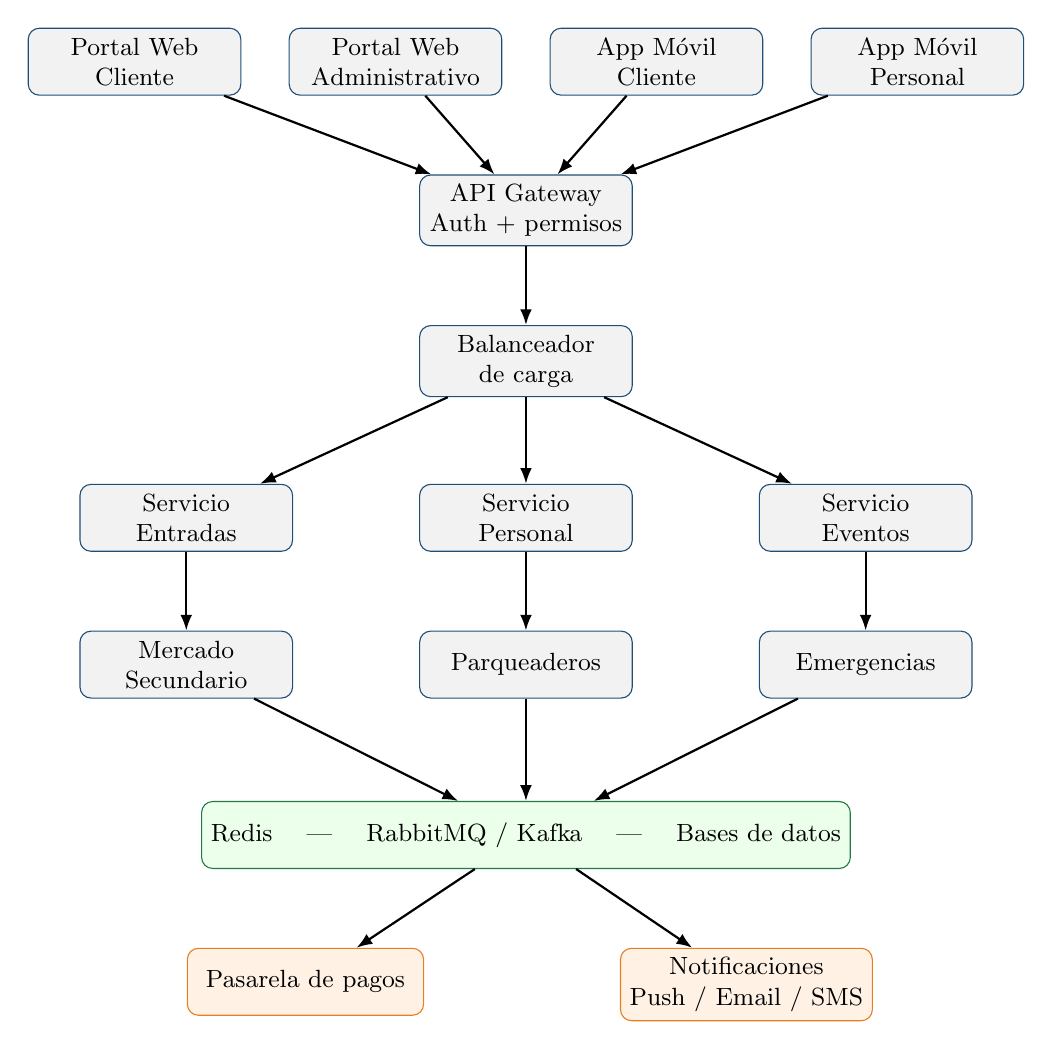
\begin{tikzpicture}[
box/.style={draw=azul,rounded corners,fill=gris,minimum width=2.7cm,minimum height=0.85cm,align=center,font=\small},
infra/.style={draw=verde,rounded corners,fill=green!8,minimum width=3cm,minimum height=0.85cm,align=center,font=\small},
ext/.style={draw=naranja,rounded corners,fill=orange!10,minimum width=3cm,minimum height=0.85cm,align=center,font=\small},
arr/.style={-{Latex[length=2mm]},thick}
]
\node[box] (wc) {Portal Web\\Cliente};
\node[box,right=6mm of wc] (wa) {Portal Web\\Administrativo};
\node[box,right=6mm of wa] (ac) {App Móvil\\Cliente};
\node[box,right=6mm of ac] (ap) {App Móvil\\Personal};

\node[box,below=10mm of $(wc.south)!0.5!(ap.south)$] (gw) {API Gateway\\Auth + permisos};
\node[box,below=of gw] (lb) {Balanceador\\de carga};

\node[box,below left=11mm and 16mm of lb] (en) {Servicio\\Entradas};
\node[box,below=11mm of lb] (pe) {Servicio\\Personal};
\node[box,below right=11mm and 16mm of lb] (ev) {Servicio\\Eventos};

\node[box,below=of en] (ms) {Mercado\\Secundario};
\node[box,below=of pe] (pa) {Parqueaderos};
\node[box,below=of ev] (em) {Emergencias};

\node[infra,below=13mm of $(ms.south)!0.5!(em.south)$] (inf) {Redis \quad | \quad RabbitMQ / Kafka \quad | \quad Bases de datos};
\node[ext,below=of inf,xshift=-28mm] (pg) {Pasarela de pagos};
\node[ext,below=of inf,xshift=28mm] (no) {Notificaciones\\Push / Email / SMS};

\foreach \x in {wc,wa,ac,ap} \draw[arr] (\x)--(gw);
\draw[arr](gw)--(lb);
\foreach \x in {en,pe,ev} \draw[arr](lb)--(\x);
\draw[arr](en)--(ms);
\draw[arr](pe)--(pa);
\draw[arr](ev)--(em);
\foreach \x in {ms,pa,em} \draw[arr](\x)--(inf);
\draw[arr](inf)--(pg);
\draw[arr](inf)--(no);
\end{tikzpicture}
}
\caption{Arquitectura general propuesta.}
\end{figure}

\subsection{API Gateway y balanceador}

El API Gateway es el punto de entrada al backend. Centraliza autenticación, autorización, validación de tokens y enrutamiento. El balanceador distribuye solicitudes entre múltiples instancias y permite mantener el servicio disponible cuando una instancia falla.

\subsection{Microservicios}

\begin{itemize}
\item \textbf{Entradas:} compra, disponibilidad, validación y gestión de entradas.
\item \textbf{Mercado secundario:} publicación, reventa, compra y transferencia de propiedad.
\item \textbf{Personal:} empleados, roles, turnos, asignaciones y asistencia.
\item \textbf{Eventos:} eventos, localidades, configuración y aforo.
\item \textbf{Parqueaderos:} reservas, espacios, ingreso, salida, cobro y ocupación.
\item \textbf{Emergencias:} incidentes, evacuaciones, zonas, rutas, alertas y seguimiento.
\end{itemize}

Cada microservicio puede disponer de su propia base de datos para reducir el acoplamiento.

\section{Infraestructura de soporte}

\subsection{Redis}

Redis se utiliza para información de acceso rápido y control de concurrencia. En el mercado secundario puede bloquear temporalmente una entrada mientras se procesa una compra, evitando que dos compradores completen simultáneamente la misma operación.

También puede apoyar información temporal de aforo, disponibilidad, sesiones y estados que requieran consultas rápidas.

\subsection{RabbitMQ / Kafka}

Las colas desacoplan operaciones asíncronas como generación de QR, notificaciones, auditoría, liquidación de pagos y propagación de alertas.

Un ejemplo es:
\[
\texttt{ENTRADA\_TRANSFERIDA}
\rightarrow
\texttt{COLA}
\rightarrow
\begin{cases}
\text{Generar QR}\\
\text{Notificar}\\
\text{Auditar}
\end{cases}
\]

\subsection{Bases de datos}

Se plantea una base de datos independiente por dominio: entradas, personal, eventos, parqueaderos, emergencias y mercado secundario. Esto reduce el acoplamiento y permite que los servicios evolucionen de forma independiente.

\section{Servicios externos}

\subsection{Pasarela de pagos}

Se utiliza para compras, reventas, reembolsos y cobros del parqueadero. La integración debe manejar respuestas exitosas, rechazos, tiempos de espera y fallos.

\subsection{Servicio de notificaciones}

Envía notificaciones push, correo y SMS cuando corresponda. Ejemplos: confirmación de compra, reventa, nuevo QR, cambios de evento, turnos, asignaciones y emergencias.

\section{Cómo la arquitectura satisface los atributos de calidad}

\subsection{Consistencia -- Alta}

Redis puede utilizarse para bloqueo temporal de entradas durante el checkout. La persistencia de la operación se realiza en el servicio correspondiente, evitando que una entrada tenga simultáneamente dos operaciones de compra válidas.

\subsection{Disponibilidad -- Alta}

El balanceador y las múltiples instancias permiten redirigir solicitudes hacia instancias sanas. Esto es especialmente importante durante ventas, ingreso masivo, validación QR y emergencias.

\subsection{Seguridad -- Alta}

El API Gateway centraliza autenticación y autorización. Se propone control de acceso basado en roles:

\begin{center}
\begin{tabular}{p{3cm}p{8cm}}
\toprule
\textbf{Rol} & \textbf{Ejemplos de permisos}\\
\midrule
Cliente & Consultar eventos, comprar y gestionar sus entradas.\\
Empleado & Consultar turnos, registrar asistencia y reportar incidentes.\\
Supervisor & Supervisar personal, aprobar cambios y operar protocolos.\\
Organizador & Gestionar eventos, personal y operación.\\
Administrador & Administrar usuarios, roles y configuración.\\
\bottomrule
\end{tabular}
\end{center}

\subsection{Rendimiento -- Alta}

El balanceador, las instancias independientes, Redis y las colas permiten distribuir la carga y ejecutar operaciones pesadas de manera asíncrona.

\subsection{Tiempo real -- Media-Alta}

Aforo, entradas, parqueaderos, personal y emergencias requieren actualizaciones cercanas al tiempo real. Redis, colas y mecanismos de comunicación en tiempo real, como WebSockets, pueden utilizarse para estos escenarios.

\subsection{Escalabilidad -- Media}

Los servicios se pueden escalar individualmente. Durante una preventa puede crecer el servicio de Entradas, mientras que durante el ingreso puede aumentar principalmente la capacidad de validación.

\subsection{Trazabilidad -- Media}

Se deben registrar operaciones como transferencias, compras, reembolsos, cambios de turno, accesos, modificaciones administrativas y emergencias.

\subsection{Usabilidad -- Baja-Media}

Cada tipo de usuario posee una interfaz especializada: cliente, personal y administración. Esto evita presentar a cada usuario funciones que no necesita.

\subsection{Mantenibilidad -- Baja-Media}

La separación en microservicios permite modificar un dominio sin modificar directamente los demás. Esto facilita pruebas, despliegues y evolución independiente.

\subsection{Portabilidad -- Baja-Media}

Los servicios del backend son consumidos mediante APIs, por lo que pueden ser utilizados desde el portal web del cliente, portal administrativo y aplicaciones móviles sin duplicar la lógica de negocio.

\section{Caso complejo: Gestión de Evacuación ante Emergencias}

Este caso de uso se propone como un proceso complejo porque integra varios dominios y requiere disponibilidad, seguridad, rendimiento, tiempo real y trazabilidad.

\subsection{Objetivo}

Permitir que un usuario autorizado active, coordine, supervise y finalice un protocolo de evacuación utilizando información de zonas, aforo, salidas, rutas y personal operativo.

\subsection{Actores}

\begin{itemize}
\item Supervisor de emergencia.
\item Organizador.
\item Personal de seguridad.
\item Personal médico.
\item Asistentes.
\item Servicio de notificaciones.
\end{itemize}

\subsection{Flujo principal}

\begin{enumerate}
\item El supervisor inicia sesión en el módulo de emergencias.
\item Selecciona ``Activar evacuación''.
\item El sistema solicita el tipo y ubicación de la emergencia.
\item El supervisor registra la información.
\item El sistema identifica las zonas potencialmente afectadas.
\item Consulta el aforo actual.
\item Identifica las salidas disponibles.
\item Determina las rutas configuradas.
\item Presenta las rutas y zonas recomendadas.
\item El supervisor confirma el protocolo.
\item El sistema notifica al personal operativo.
\item El sistema envía instrucciones a los asistentes.
\item El sistema monitorea las zonas.
\item El supervisor consulta el avance y atiende alertas.
\item El supervisor confirma la finalización y el sistema registra la emergencia.
\end{enumerate}

\subsection{Flujos alternativos}

\textbf{Ruta bloqueada:} si una salida deja de estar disponible, el sistema la retira de las rutas recomendadas, busca una alternativa y actualiza las instrucciones.

\textbf{Zona congestionada:} el sistema genera una alerta y el supervisor puede seleccionar una ruta alternativa.

\textbf{Evacuación parcial:} solamente se notifican y controlan las zonas afectadas.

\textbf{Cambio del nivel de emergencia:} el sistema vuelve a evaluar zonas y rutas cuando aumenta la gravedad.

\subsection{Excepciones}

\begin{itemize}
\item No existen rutas disponibles.
\item Se pierde comunicación con el monitoreo.
\item Falla el servicio de notificaciones.
\item El usuario no tiene permisos.
\item Se pierde temporalmente la conexión de una aplicación.
\end{itemize}

\subsection{Atributos de calidad del caso}

\begin{itemize}
\item \textbf{Disponibilidad:} el servicio debe permanecer operativo durante la emergencia.
\item \textbf{Rendimiento:} las alertas deben procesarse rápidamente.
\item \textbf{Tiempo real:} el estado de las zonas debe actualizarse con baja latencia.
\item \textbf{Seguridad:} solo usuarios autorizados pueden activar o modificar el protocolo.
\item \textbf{Trazabilidad:} las acciones deben quedar registradas.
\end{itemize}

\section{Comunicación durante una emergencia}

Un escenario representativo es un concierto en el que se detecta un incendio en una zona. El supervisor activa el protocolo desde el portal administrativo. El servicio de emergencias consulta aforo, zonas y rutas y publica eventos para notificar al personal y a los asistentes.

\begin{center}
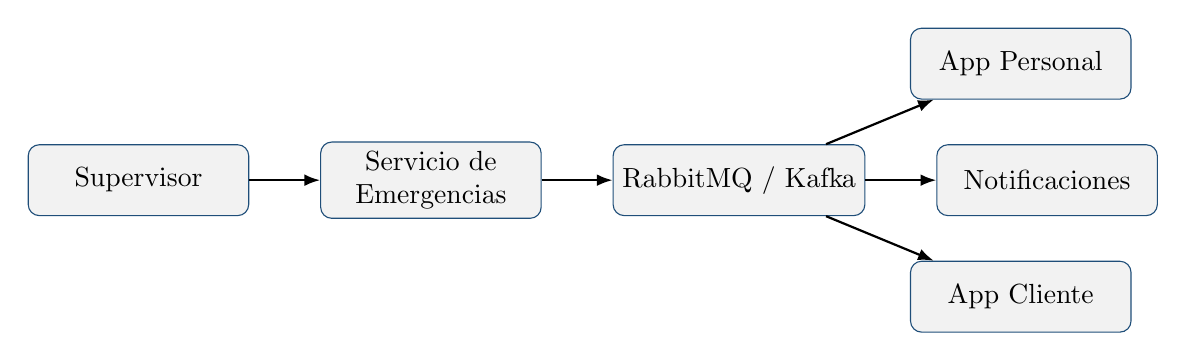
\begin{tikzpicture}[
box/.style={draw=azul,rounded corners,fill=gris,minimum width=2.8cm,minimum height=0.9cm,align=center},
arr/.style={-{Latex[length=2mm]},thick}
]
\node[box] (s) {Supervisor};
\node[box,right=9mm of s] (e) {Servicio de\\Emergencias};
\node[box,right=9mm of e] (q) {RabbitMQ / Kafka};
\node[box,above right=8mm of q] (p) {App Personal};
\node[box,below right=8mm of q] (c) {App Cliente};
\node[box,right=9mm of q] (n) {Notificaciones};
\draw[arr](s)--(e);
\draw[arr](e)--(q);
\draw[arr](q)--(p);
\draw[arr](q)--(c);
\draw[arr](q)--(n);
\end{tikzpicture}
\end{center}

\section{Relación entre interfaces y microservicios}

\begin{longtable}{p{4cm}p{4cm}p{6cm}}
\toprule
\textbf{Servicio} & \textbf{Interfaces} & \textbf{Responsabilidad}\\
\midrule
Entradas & Web Cliente, App Cliente & Compra, disponibilidad, validación y gestión.\\
Mercado Secundario & Web Cliente & Publicación, compra y transferencia.\\
Personal & Web Administrativo, App Personal & Empleados, turnos, asignaciones y asistencia.\\
Eventos & Web Administrativo, Web Cliente, Apps & Gestión y consulta de eventos.\\
Parqueaderos & Web Cliente, Web Administrativo, Apps & Reservas, espacios, cobros y ocupación.\\
Emergencias & Web Administrativo, App Personal, App Cliente & Activación, coordinación, alertas y seguimiento.\\
\bottomrule
\end{longtable}

\section{Resumen de decisiones arquitectónicas}

\begin{table}[H]
\centering
\small
\begin{tabular}{p{4cm}p{5cm}p{5cm}}
\toprule
\textbf{Decisión} & \textbf{Problema} & \textbf{Atributos}\\
\midrule
Microservicios & Separación de dominios y escalamiento & Escalabilidad, mantenibilidad, rendimiento\\
API Gateway & Punto central de acceso y seguridad & Seguridad, mantenibilidad\\
Balanceador & Distribución de solicitudes & Disponibilidad, rendimiento\\
Redis & Acceso rápido y bloqueo temporal & Consistencia, tiempo real, rendimiento\\
RabbitMQ/Kafka & Procesamiento asíncrono & Rendimiento, escalabilidad\\
BD por servicio & Evitar acoplamiento de datos & Mantenibilidad, escalabilidad\\
Notificaciones & Comunicación desacoplada & Rendimiento, tiempo real\\
Pasarela de pagos & Transacciones externas & Seguridad, consistencia\\
Interfaces especializadas & Adaptación al usuario & Usabilidad, portabilidad\\
\bottomrule
\end{tabular}
\caption{Resumen de decisiones arquitectónicas.}
\end{table}

\section{Conclusión}

La arquitectura propuesta conserva las decisiones fundamentales de la primera versión, pero las adapta a una definición más concreta del sistema: un portal web para clientes, un portal web administrativo y operativo, una aplicación móvil para clientes y una aplicación móvil para el personal.

La separación de interfaces permite que cada tipo de usuario tenga las funcionalidades que necesita, mientras que el backend mantiene la lógica de negocio centralizada en servicios independientes.

Los atributos de calidad prioritarios siguen siendo consistencia, disponibilidad, seguridad y rendimiento. Estos se soportan mediante microservicios, API Gateway, balanceador de carga, Redis, colas de mensajes, bases de datos independientes y servicios externos de pago y notificaciones.

La incorporación de aplicaciones móviles aumenta la importancia de tiempo real, usabilidad y portabilidad. Asimismo, la gestión de evacuación ante emergencias constituye un caso complejo adecuado para demostrar cómo las decisiones arquitectónicas responden a atributos de calidad concretos.

\end{document}
